\documentclass[12pt,a4paper]{article}

\usepackage[utf8]{inputenc}
\usepackage[T1]{fontenc}
\usepackage[brazilian]{babel}
\usepackage{geometry}
\usepackage{setspace}
\usepackage{graphicx}
\usepackage{booktabs}
\usepackage{array}
\usepackage{tabularx}
\usepackage{siunitx}
\usepackage{amsmath}
\usepackage{float}
\usepackage{placeins}
\usepackage{caption}
\usepackage{subcaption}
\usepackage{pgfplots}
\usepackage{hyperref}
\usepackage{xcolor}

\geometry{margin=2.5cm}
\onehalfspacing
\pgfplotsset{compat=1.18}
\sisetup{
  separate-uncertainty=true,
  per-mode=symbol,
  detect-all
}

\newcommand{\todo}[1]{\textcolor{red}{[PREENCHER: #1]}}
\newcommand{\blank}{\todo{preencher}}
\newcolumntype{Y}{>{\raggedright\arraybackslash}X}
\newcolumntype{Z}{>{\centering\arraybackslash}X}

\title{Relatorio 2: A Mini Central Termeletrica}
\author{\todo{Seu nome}\\\todo{Integrantes do grupo}}
\date{HID-31: Fenomenos de Transporte\\\today}

\begin{document}

\begin{titlepage}
  \centering
  {\large Instituto Tecnologico de Aeronautica\par}
  {\large Divisao de Engenharia Civil\par}
  \vspace{2cm}
  {\Large\bfseries Relatorio 2\par}
  \vspace{0.4cm}
  {\Large A Mini Central Termeletrica\par}
  \vspace{2cm}
  {\large HID-31: Fenomenos de Transporte\par}
  {\large Data do laboratorio: \todo{dia mes 2026}\par}
  \vfill
  {\large Alunos:\par}
  \todo{Seu nome}\\
  \todo{Integrantes do grupo}
  \vfill
  {\large Sao Jose dos Campos, \today\par}
\end{titlepage}

\tableofcontents
\newpage

\section{Introducao}

Este relatorio estuda a operacao de uma mini central termeletrica composta por um gerador de vapor, uma turbina e um gerador eletrico conectado a cargas eletricas. O experimento mede tensao e corrente para diferentes ajustes de carga e pressoes de vapor. A potencia eletrica e calculada por \(P = VI\), e os resultados sao usados para analisar como a carga e a pressao afetam o desempenho do gerador.

\todo{Depois de completar o laboratorio, substitua este paragrafo por um resumo curto dos principais resultados numericos e conclusoes.}

\section{Objetivo}

O objetivo desta atividade de laboratorio e observar a operacao de um pequeno sistema de geracao termeletrica e medir como a tensao, a corrente e a potencia eletrica variam com a carga e com a pressao de vapor.

\section{Montagem Experimental}

A mini central possui tres subsistemas principais:

\begin{itemize}
  \item \textbf{Gerador de vapor:} queimador, caldeira, indicador de nivel da agua, valvula de seguranca e manometro da caldeira.
  \item \textbf{Turbina:} entrada de vapor, rotor da turbina e exaustao do condensado.
  \item \textbf{Gerador eletrico e sistema de cargas:} gerador, banco de lampadas, reostato, voltimetro, amperimetro e controles de carga.
\end{itemize}

\begin{figure}[H]
  \centering
  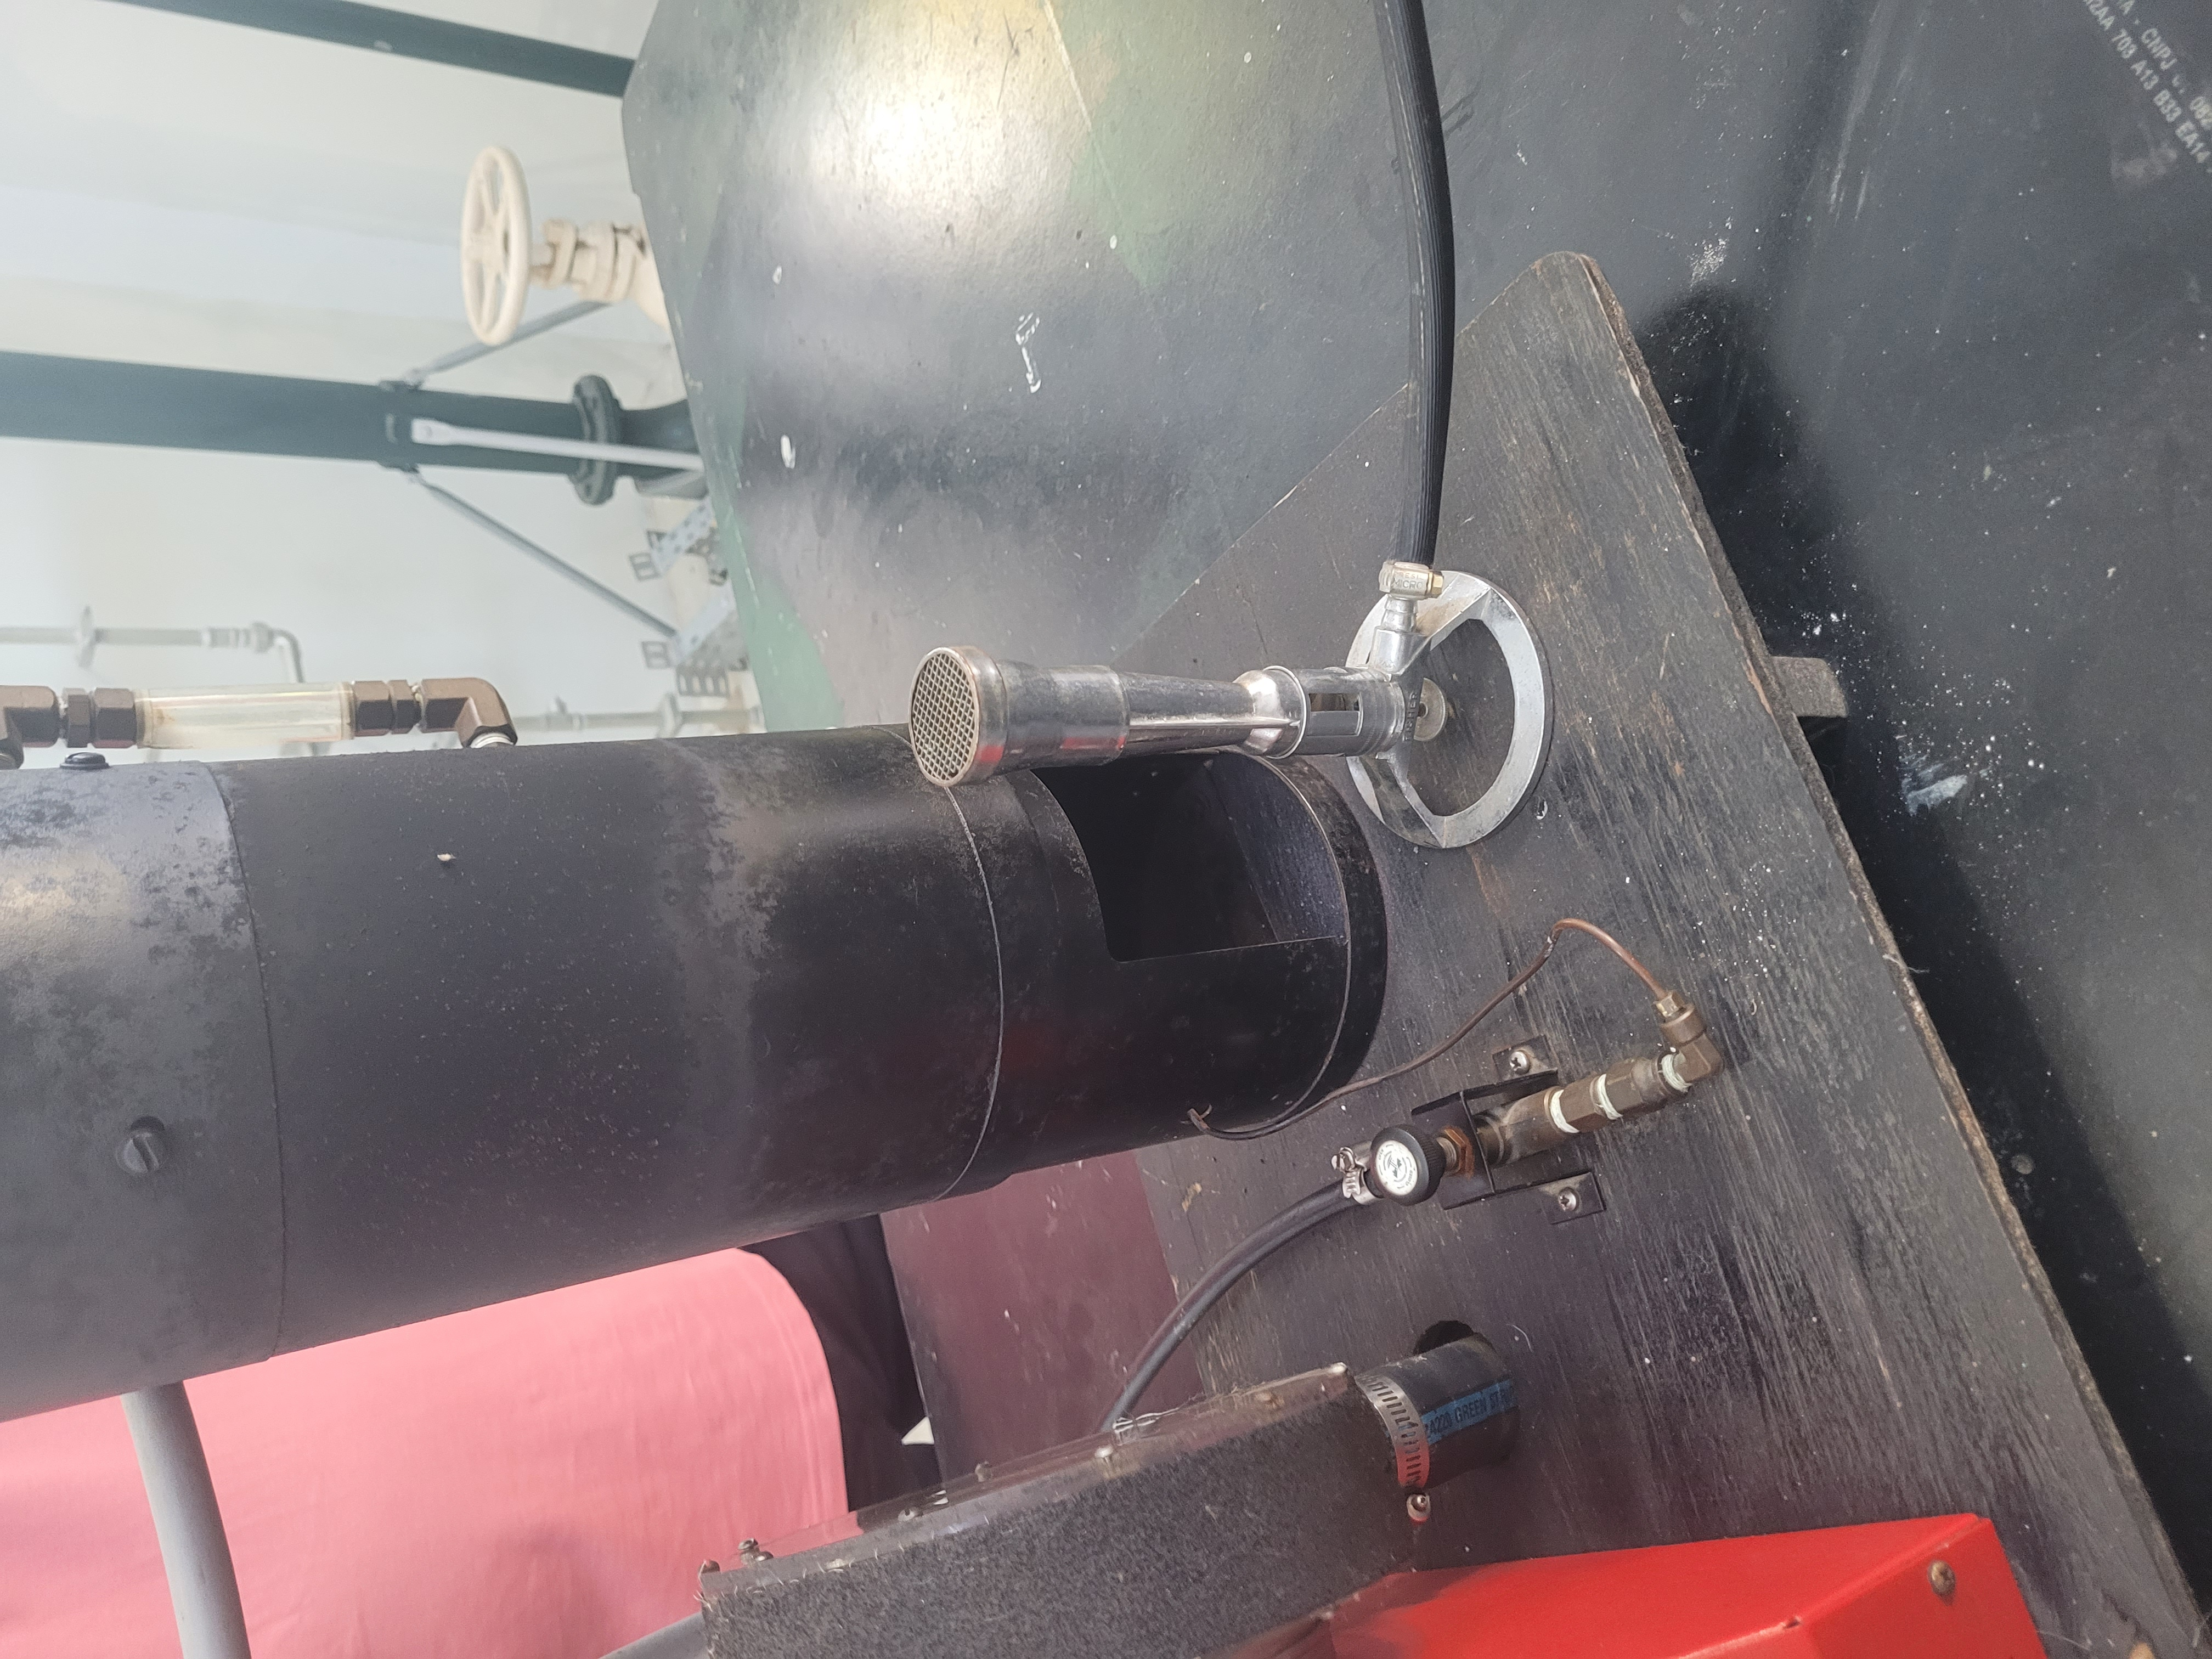
\includegraphics[angle=-90,width=0.65\textwidth]{20260507_154152.jpg}
  \caption{Mini central termeletrica usada no experimento.}
  \label{fig:setup}
\end{figure}

\section{Teoria}

A potencia eletrica de saida e calculada a partir da tensao e da corrente medidas:

\begin{equation}
  P = VI,
  \label{eq:power}
\end{equation}

em que \(P\) e a potencia eletrica em watts (\si{\watt}), \(V\) e a tensao em volts (\si{\volt}) e \(I\) e a corrente em amperes (\si{\ampere}).

Para uma carga resistiva, a lei de Ohm fornece

\begin{equation}
  V = RI.
  \label{eq:ohm}
\end{equation}

Combinando as Equacoes~\ref{eq:power} e~\ref{eq:ohm}, a potencia tambem pode ser escrita como

\begin{equation}
  P = \frac{V^2}{R} = I^2R.
  \label{eq:resistive-power}
\end{equation}

Essa relacao ajuda a explicar o experimento com as lampadas: ao mudar a resistencia equivalente, muda-se a corrente exigida do gerador. Se o gerador nao consegue manter a mesma tensao sob maior carga, a tensao terminal pode diminuir.

\section{Procedimento}

\subsection{Experimento I: Banco de Lampadas}

Inicialmente, o gerador de vapor foi colocado em funcionamento para produzir o vapor necessario ao acionamento da turbina. Apos a estabilizacao inicial do sistema, a turbina foi acionada e passou a converter parte da energia do vapor em movimento de rotacao.

Com a turbina em movimento, o gerador eletrico foi conectado ao banco de lampadas. Em seguida, as chaves das lampadas foram acionadas gradualmente. A cada nova lampada conectada, observou-se a mudanca no brilho do conjunto, pois o aumento da carga eletrica altera a corrente exigida do gerador. As observacoes qualitativas foram registradas para comparar o comportamento do sistema com diferentes resistencias equivalentes.

\subsection{Experimento II: Carga com Reostato}

Na segunda parte do experimento, utilizou-se o circuito com reostato para controlar a carga eletrica aplicada ao gerador. O sistema foi operado primeiro com pressao de vapor de \SI{40}{psi}. Para essa condicao, ajustou-se a carga em 0, 20, 40, 60, 80 e 100 por cento. Em cada ajuste, foram lidas a tensao nos terminais do gerador e a corrente eletrica no circuito.

Depois de completar as medicoes em \SI{40}{psi}, o procedimento foi repetido para a pressao de \SI{50}{psi}. Os mesmos valores de ajuste de carga foram utilizados, permitindo comparar o desempenho eletrico da mini central em duas condicoes de pressao. Com os valores medidos de tensao e corrente, calculou-se a potencia eletrica de saida por meio da relacao \(P = VI\).

\section{Resultados}

\subsection{Observacoes do Experimento I}

\begin{table}[H]
  \centering
  \caption{Observacoes qualitativas do experimento com lampadas.}
  \label{tab:lamp-observations}
  \begin{tabularx}{\textwidth}{YY}
    \toprule
    Condicao & Observacao \\
    \midrule
    Lampadas iniciais ligadas & \blank \\
    Mais lampadas conectadas & \blank \\
    Condicao final & \blank \\
    \bottomrule
  \end{tabularx}
\end{table}

\subsection{Medidas do Experimento II}

\begin{table}[H]
  \centering
  \caption{Medidas em \SI{40}{psi}. Calcular a potencia usando \(P=VI\).}
  \label{tab:40psi}
  \begin{tabular}{S[table-format=3.0] S[table-format=2.3] S[table-format=3.2] S[table-format=3.2]}
    \toprule
    {Carga (\%)} & {Corrente (\si{\ampere})} & {Tensao (\si{\volt})} & {Potencia (\si{\watt})} \\
    \midrule
    0   & {} & {} & {} \\
    20  & {} & {} & {} \\
    40  & {} & {} & {} \\
    60  & {} & {} & {} \\
    80  & {} & {} & {} \\
    100 & {} & {} & {} \\
    \bottomrule
  \end{tabular}
\end{table}

\begin{table}[H]
  \centering
  \caption{Medidas em \SI{50}{psi}. Calcular a potencia usando \(P=VI\).}
  \label{tab:50psi}
  \begin{tabular}{S[table-format=3.0] S[table-format=2.3] S[table-format=3.2] S[table-format=3.2]}
    \toprule
    {Carga (\%)} & {Corrente (\si{\ampere})} & {Tensao (\si{\volt})} & {Potencia (\si{\watt})} \\
    \midrule
    0   & 0.15 & 9.3  & 1.34 \\
    20  & 0.20 & 11.1 & 2.22 \\
    40  & 0.25 & 10.5 & 2.63 \\
    60  & 0.31 & 9.5  & 2.95 \\
    80  & 0.50 & 5.5  & 2.75 \\
    100 & 0.51 & 1.1  & 0.56 \\
    \bottomrule
  \end{tabular}
\end{table}

\section{Graficos}

Os graficos a seguir foram construidos com as medidas obtidas para a pressao de \SI{50}{psi}.

\subsection{Tensao em Funcao da Potencia Eletrica}

\begin{figure}[H]
  \centering
  \begin{tikzpicture}
    \begin{axis}[
      width=0.9\textwidth,
      height=0.5\textwidth,
      xlabel={Potencia eletrica, \(P\) (\si{\watt})},
      ylabel={Tensao, \(V\) (\si{\volt})},
      grid=both,
      legend pos=best
    ]
      \addplot[mark=square, thick] coordinates {
        (0.56,1.1)
        (1.34,9.3)
        (2.22,11.1)
        (2.63,10.5)
        (2.75,5.5)
        (2.95,9.5)
      };
      \addlegendentry{\SI{50}{psi}}
    \end{axis}
  \end{tikzpicture}
  \caption{Tensao em funcao da potencia eletrica para pressao de \SI{50}{psi}.}
  \label{fig:voltage-power}
\end{figure}

\subsection{Potencia Eletrica em Funcao da Corrente}

\begin{figure}[H]
  \centering
  \begin{tikzpicture}
    \begin{axis}[
      width=0.9\textwidth,
      height=0.5\textwidth,
      xlabel={Corrente, \(I\) (\si{\ampere})},
      ylabel={Potencia eletrica, \(P\) (\si{\watt})},
      grid=both,
      legend pos=best
    ]
      \addplot[mark=square, thick] coordinates {
        (0.15,1.34)
        (0.20,2.22)
        (0.25,2.63)
        (0.31,2.95)
        (0.50,2.75)
        (0.51,0.56)
      };
      \addlegendentry{\SI{50}{psi}}
    \end{axis}
  \end{tikzpicture}
  \caption{Potencia eletrica em funcao da corrente para pressao de \SI{50}{psi}.}
  \label{fig:power-current}
\end{figure}

\subsection{Potencia Eletrica em Funcao da Carga}

\begin{figure}[H]
  \centering
  \begin{tikzpicture}
    \begin{axis}[
      width=0.9\textwidth,
      height=0.5\textwidth,
      xlabel={Ajuste de carga (\%)},
      ylabel={Potencia eletrica, \(P\) (\si{\watt})},
      grid=both,
      legend pos=best,
      xmin=0,
      xmax=100
    ]
      \addplot[mark=square, thick] coordinates {
        (0,1.34)
        (20,2.22)
        (40,2.63)
        (60,2.95)
        (80,2.75)
        (100,0.56)
      };
      \addlegendentry{\SI{50}{psi}}
    \end{axis}
  \end{tikzpicture}
  \caption{Potencia eletrica em funcao do ajuste de carga do reostato para pressao de \SI{50}{psi}.}
  \label{fig:power-load}
\end{figure}

\section{Discussao}

\subsection{Experimento com Lampadas}

No experimento com o banco de lampadas, o brilho variou conforme novas lampadas foram conectadas ao circuito. Isso ocorreu porque a resistencia equivalente do conjunto mudou, alterando a corrente exigida do gerador. Para uma carga resistiva, a potencia eletrica pode ser relacionada com a tensao por \(P = V^2/R\). Assim, quando a resistencia equivalente diminui, a corrente tende a aumentar.

Entretanto, uma resistencia menor nao significa necessariamente maior potencia real fornecida pelo sistema. Em um caso ideal, a reducao da resistencia poderia aumentar a potencia. Na pratica, o gerador possui limitacoes mecanicas e eletricas. Quando a carga aumenta muito, a turbina pode perder rotacao e a tensao nos terminais pode cair. Por isso, o brilho das lampadas depende nao apenas da resistencia, mas tambem da capacidade do gerador de manter tensao e corrente.

\subsection{Experimento com Reostato}

No ensaio com reostato, os dados obtidos para \SI{50}{psi} mostram que a potencia eletrica aumentou inicialmente com o ajuste de carga. A potencia passou de \SI{1.34}{W}, com carga de 0\%, para o valor maximo de \SI{2.95}{W}, com carga de 60\%. Depois desse ponto, a potencia diminuiu, chegando a \SI{0.56}{W} com carga de 100\%.

Esse comportamento indica que existe uma condicao intermediaria de carga em que o sistema opera melhor. Em cargas muito baixas, a corrente e pequena, e por isso a potencia tambem e limitada. Em cargas muito altas, a corrente aumenta, mas a tensao cai de forma significativa. Essa queda de tensao pode ser explicada pelas perdas internas do gerador, pelo maior esforco mecanico exigido da turbina e por possiveis variacoes na pressao e na vazao de vapor.

As incertezas experimentais tambem influenciam os resultados. Entre as principais fontes de erro estao a leitura dos instrumentos analogicos ou digitais, a estabilidade da pressao de vapor, a variacao da rotacao da turbina e o ajuste manual do reostato. Mesmo assim, os dados permitem observar claramente a relacao entre carga, tensao, corrente e potencia eletrica.

\section{Conclusao}

O experimento permitiu observar o funcionamento de uma mini central termeletrica, na qual a energia termica do vapor foi convertida em energia mecanica na turbina e, em seguida, em energia eletrica no gerador. No ensaio com reostato a \SI{50}{psi}, a maior potencia eletrica medida foi de \SI{2.95}{W}, obtida com ajuste de carga de 60\%. Para cargas maiores, a potencia diminuiu devido a queda da tensao nos terminais do gerador. Esse resultado mostra que o desempenho do sistema depende do equilibrio entre tensao e corrente, e nao apenas do aumento da carga eletrica. A atividade tambem evidenciou a importancia de controlar a pressao de vapor, a rotacao da turbina e as condicoes de medicao para obter resultados mais consistentes.

\section*{Referencias}

\begin{itemize}
  \item Roteiro do Laboratorio 2 de HID-31, \textit{A Mini Central Termeletrica}, Instituto Tecnologico de Aeronautica, 2026.
\end{itemize}

\end{document}
